\documentclass[10pt]{article}
\usepackage[utf8]{inputenc}
\usepackage[margin=2.5cm]{geometry}

% packages die oefters gebraucht werden
\usepackage{amsmath, amssymb}
\usepackage{graphicx}
\usepackage{fancyhdr}
\usepackage{aligned-overset}
\usepackage{float}
\usepackage{wrapfig}

\fancyhf{}
% vspaces in den headern fuer Distanzen notwendig
% linke Seite: Namen der Abgabegruppe
\lhead{\textbf{Matthias Maile}\vspace{0.5cm}}
% rechte Seite: Modul, Gruppe, Semester
\rhead{\textbf{Höhere Mathematik II\\Sommersemester 2020}\vspace{0.5cm}}
% Center: nr. des blattes
\chead{\vspace{1.5cm}\huge{\textbf{7. Übungsblatt}}}
% benoetigt damit der eigentliche Text nicht in der Überschrift steckt
\setlength{\headheight}{3cm} 

% custom commands
\newcommand{\arsinh}{\text{arsinh}}

% for newpage to reset headheight
\newcommand{\secondpage}{
	\newpage 
	\setlength{\headheight}{0cm}
}

\begin{document}
\thispagestyle{fancy}
\section*{Aufgabe 25}


\section*{Aufgabe 26}
a) Gemäß der Grafik Teile ich das Gebiet $D$ in $A$ und $B$ auf, und 
integriere diese einzeln.
\begin{wrapfigure}{r}{0.3\textwidth}
	\centering
	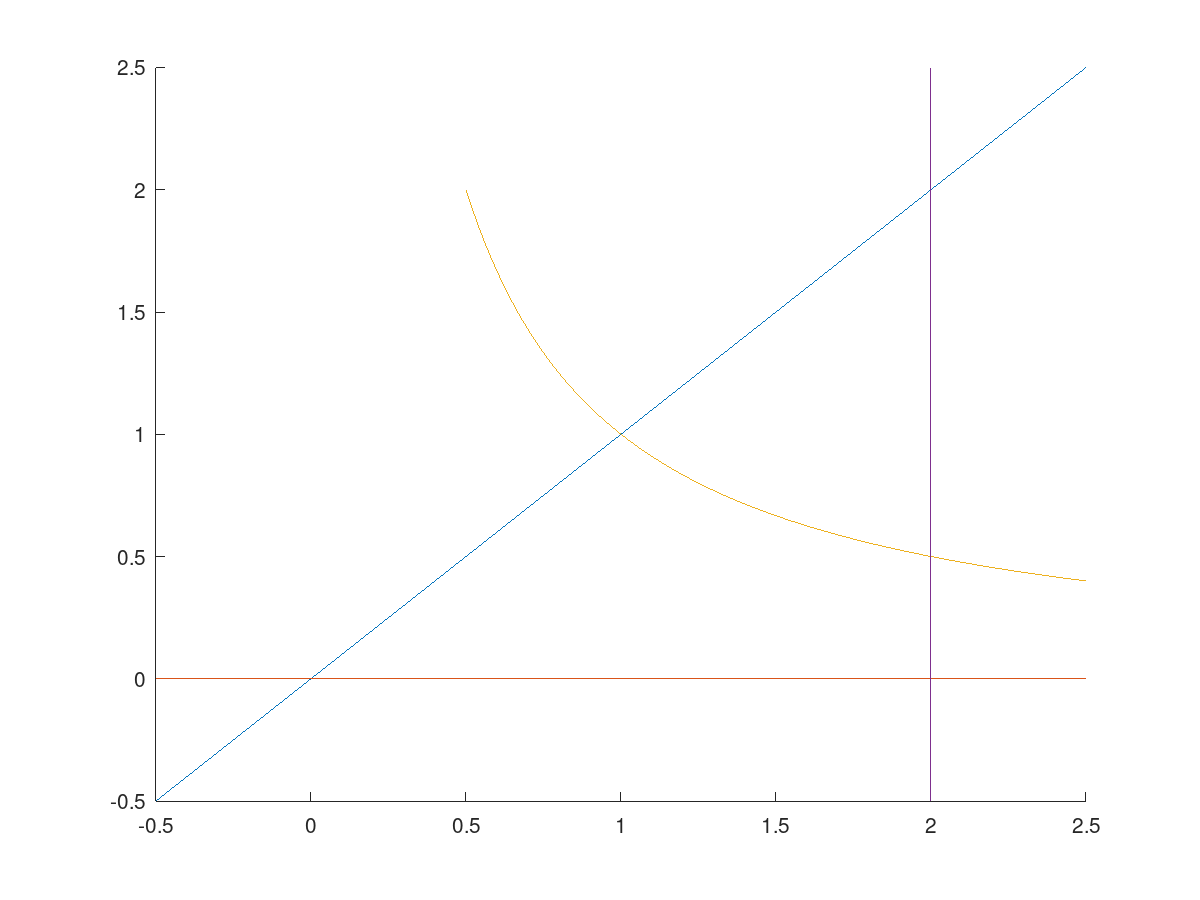
\includegraphics[width=5cm]{26-plt.png}
\end{wrapfigure}

\begin{align*}
	\int_D \frac{y^2}{x^2} d(x,y) 
	% aufteilen der flaeche
	&= \int_A \frac{y^2}{x^2} d(x,y) +\int_B \frac{y^2}{x^2} d(x,y) \\
	% integrationsgrenzen
	&= \int_0^1 \int_0^x \frac{y^2}{x^2} \ dy \ dx
	+ \int_1^2 \int_0^{\frac1x} \frac{y^2}{x^2} \ dy \ dx \\
	% nac y integrieren
	&= \int_0^1 \frac1{x^2} \left[ \frac{y^3}{3} \right]_0^x \ dx
	+ \int_1^2 \frac1{x^2} 
	\left[ \frac{y^3}{3} \right]_0^{\frac1x} \ dx \\
	% y einsetzen
	&= \int_0^1 \frac1{x^2}\frac{x^3}{3} \ dx
	+ \int_1^2 \frac1{x^2} 
	\frac{1}{3x^3} \ dx \\
	% vereinfachen
	&= \int_0^1 \frac x3 \ dx
	+ \int_1^2 \frac{1}{3x^5} \ dx \\
	% nach x integrieren
	&= \left[ \frac{x^2}{6} \right]_0^1
	+ \frac13 \left[ \frac{-1}{4x^4} \right]_1^2 \\
	% einsetzen
	&= \frac16 + \frac 1{12} - \frac{1}{12} \frac1{16} \\
	% ausrechen
	&= \frac{47}{16} \frac{1}{12}
\end{align*}


\end{document}
